\input ../SlidePreamble
\input ../preamble


\begin{document}

{\Huge

  \centerline{\bf TTIC 31230, Fundamentals of Deep Learning}
  \bigskip
  \centerline{David McAllester, April 2019}
  \vfill
  \centerline{\bf Interpreting Deep Networks}
  \vfill
  \centerline{\bf The Black Box Problem}
  \vfill  
  \vfill

\slide{The Human Black Box --- Perception}

Introspection is notoriously inadequate for AI.

\vfill
Explain how you know there are upside down glasses in this picture.
\vfill
\centerline{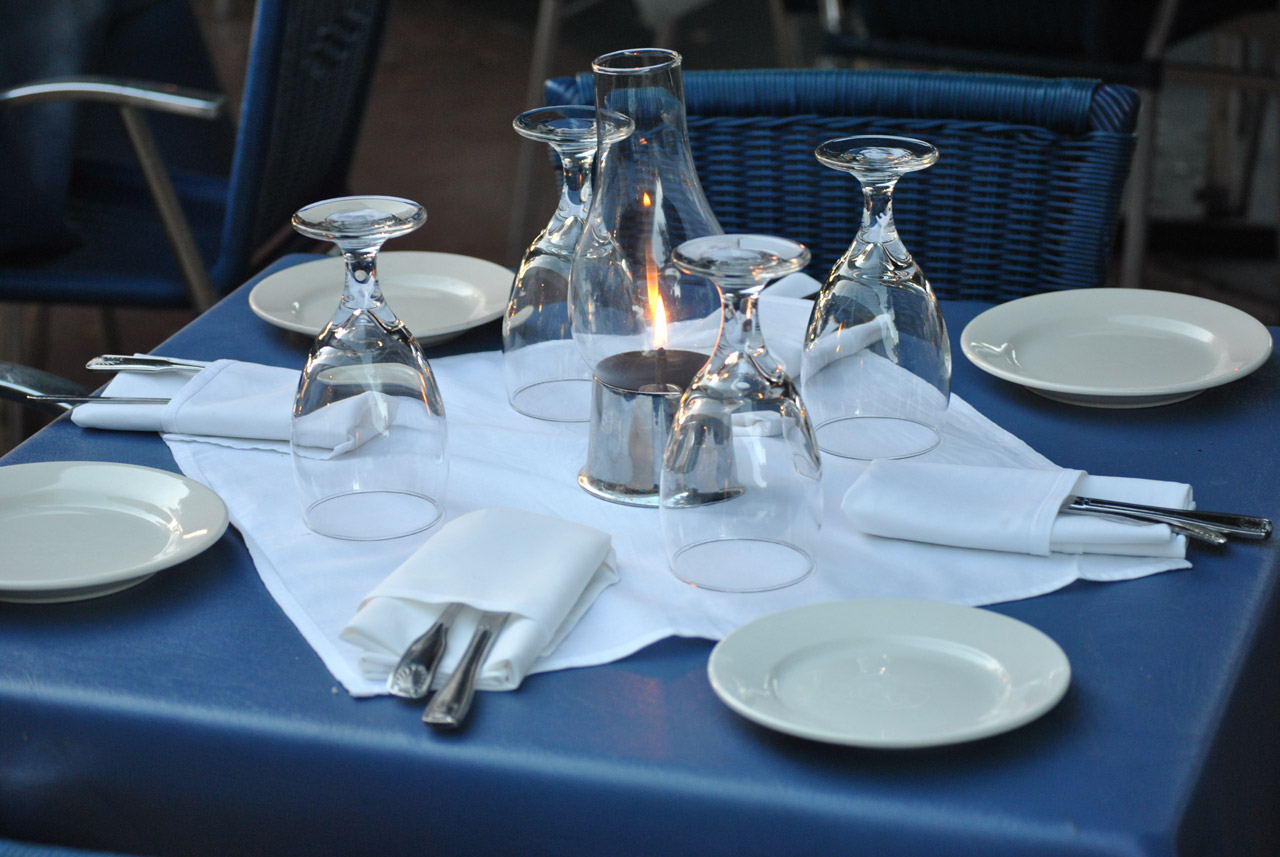
\includegraphics[height = 3.5in]{../images/table-setting}}

\slide{The Human Black Box --- Inference}

Certain facts are obvious.

\vfill
A king on empty chess board can reach every square (obvious).

\vfill
A knight on an empty chess board can reach every square (true but not obvious).

\slide{The Human Black Box --- Inference}

Consider a graph with colored nodes.

\vfill
If every edge is between nodes of the same color, then any path connects nodes of the same color.

\vfill
Consider a swiss chocolate bar of $3 \times 5$ little squares.

\vfill
How many breaks does it take to reduce this to fifteen unconnected squares?

\slide{Dimensionality Reduction}

\centerline{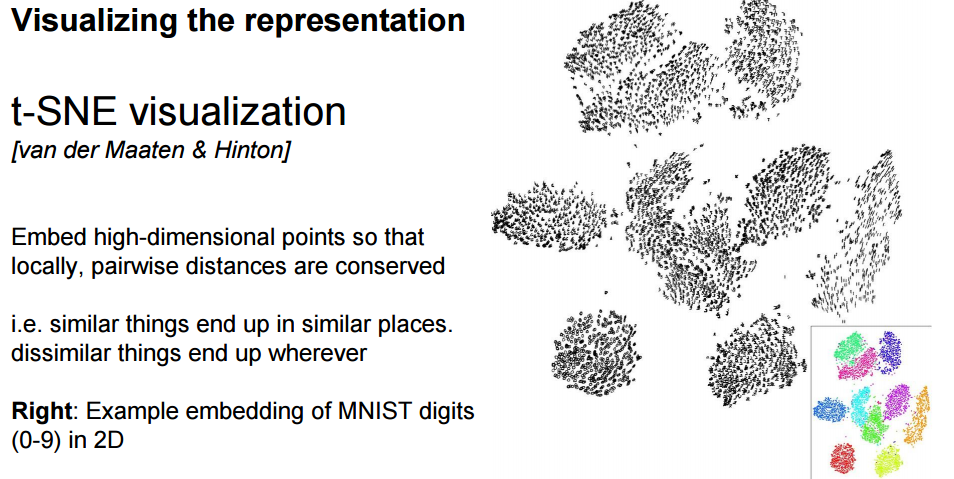
\includegraphics[width = 9.5in]{../images/t-SNE}}
\centerline{[Stanford CS231]}

\slide{t-SNE}
Consider high dimensional data $x_1,\;\ldots,\;x_N$ with $x \in \mathbb{R}^d$.

\vfill
$$P(j|i) = \frac{1}{Z_i} \exp\left(\frac{-||x_i -x_j||^2}{2\sigma_i^2}\right)$$

\vfill
Set $\sigma_i$ such that $H(P(j|i)) = \ln k$ (soft $k$ nearest neighbors).

\vfill
$$P(i,j) = P(i)P(j|i) = \frac{1}{N}\;P(j|i)$$

\slide{t-SNE}
Let $Y = \{y_i\ldots,y_N\}$ be an assignment of a vector with $y_i \in \mathbb{R}^2$ to each high dimensional point $x_i$.

\vfill
$$Q_Y(i,j) = \frac{1}{Z}\;\left(\frac{1}{1 + ||y_i -y_j||^2}\right)$$

\vfill
$$Y^* = \argmin_Y \;\mathrm{KL}(P,Q_Y)$$

\slide{t-SNE vs. Projection Modeling}

t-SNE --- $y(x)$ is defined by a table on the data points.

\vfill
In PCA or Isomap we have $y_\Phi(x) \in \mathbb{R}^2$ for a parameterized function $y_\Phi$.

\slide{Visualizing the Filters}

\centerline{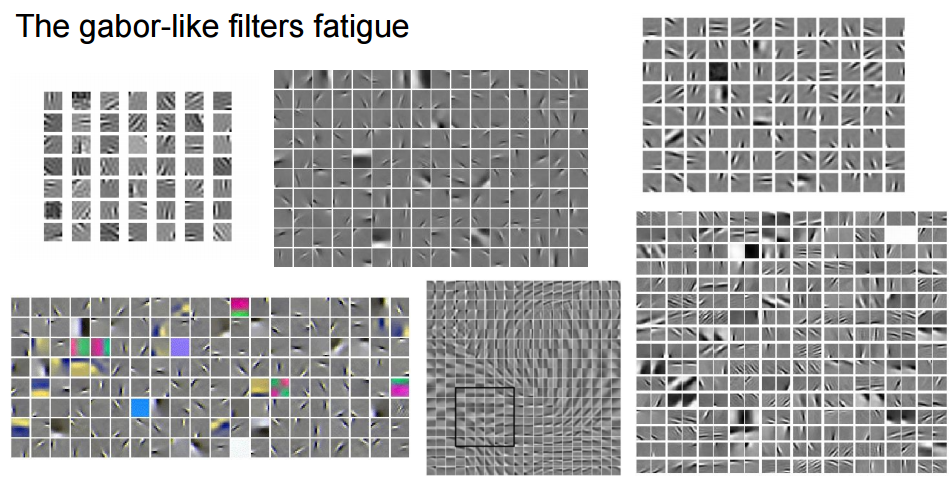
\includegraphics[width = 9.5in]{../images/Filters}}
\centerline{[Stanford CS231]}

\slide{}

\centerline{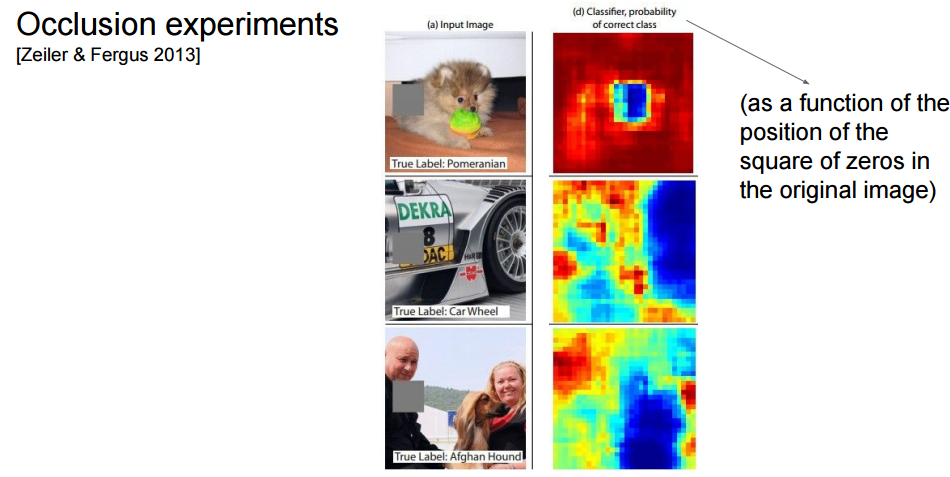
\includegraphics[width = 9.5in]{../images/Occlusion}}
\centerline{[Stanford CS231]}

\slide{Backpropagation from Individual Neurons}

\centerline{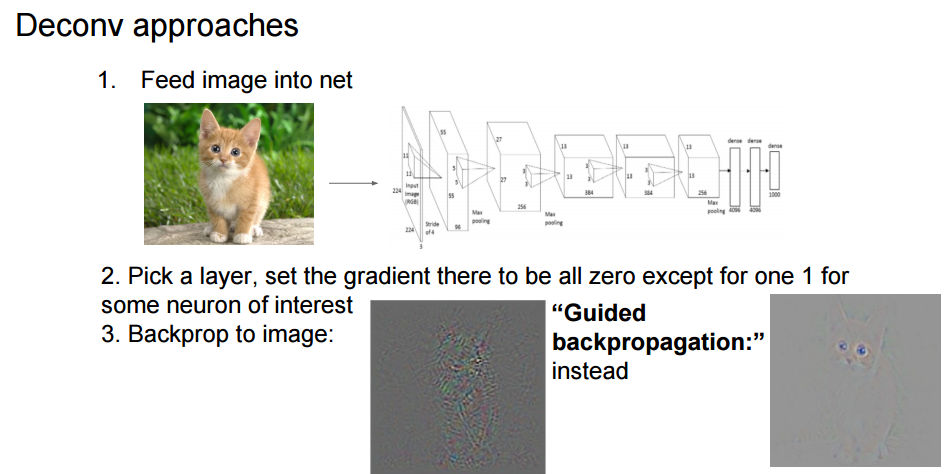
\includegraphics[width = 9.5in]{../images/DeconvAnalysis}}
\centerline{[Stanford CS231]}

\slide{Guided Backpropagation}

Rather than $\partial \ell/ \partial x$ we are interested in $\partial \mathrm{neuron}/\partial x$.

\vfill
We are interested in $\partial \mathrm{neuron}/\partial x$ where $x$ in one color channel of one input pixel.

\vfill
It turns out that $\partial \mathrm{neuron}/\partial x$ looks like image noise.

\vfill
Instead we compute $x$.ggrad  --- a {\bf guided} version of $\partial \mathrm{neuron}/\partial x$.

\slide{Guided Backpropagation}

\vfill
Guided backpropagation only considers computation paths that activate (as opposed to suppress) the neuron all along the activation path.

\vfill
The backpropagation at activation functions is modified.

\vfill
For a neuron $y$ with $y = s(x)$ for activation function $s$:

$$x.\mathrm{ggrad} = \mathbf{1}[y.\mathrm{ggrad} > 0] \;y.\mathrm{ggrad}\; ds/dx$$


\slide{Guided Backpropagation}

\centerline{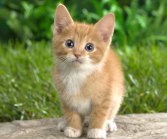
\includegraphics[width = 6in]{../images/DeconvKitten}}

\slide{Guided Backpropagation}

\centerline{[Zeigler and Fergus 2013]}

\centerline{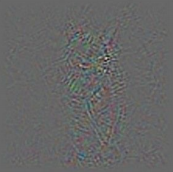
\includegraphics[width = 4in]{../images/DeconvUnguided} \hfill 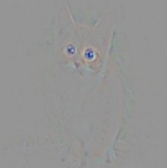
\includegraphics[width=4in]{../images/DeconvGuided}}

\centerline{[Zeigler and Fergus 2013]}

\slide{Neural Network Neuroscience}

\centerline{[Zeigler and Fergus 2013]}

\vfill
Take a neuron (linear threshold unit) and select the images causing the greatest response of that Neuron.

\vfill
Do guided backpropagation from that neuron onto the image.

\slide{Guided Backpropagation Layer 2}

\centerline{\includegraphics[width = 8in]{../images/Deconv2IM}}

\centerline{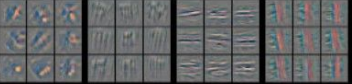
\includegraphics[width = 8in]{../images/Deconv2}}

\centerline{[Zeigler and Fergus 2013]}

\slide{Guided Backpropagation Layer 3}

\centerline{\includegraphics[width = 8in]{../images/Deconv3IM}}

\centerline{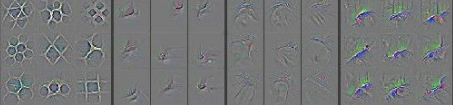
\includegraphics[width = 8in]{../images/Deconv3}}

\centerline{[Zeigler and Fergus 2013]}

\slide{Guided Backpropagation Layer 4}

\centerline{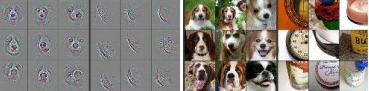
\includegraphics[width = 8in]{../images/Deconv4a}}

\centerline{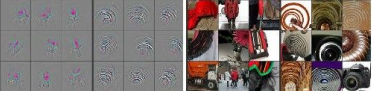
\includegraphics[width = 8in]{../images/Deconv4b}}

\centerline{[Zeigler and Fergus 2013]}


\slide{Guided Backpropagation Layer 5}

\centerline{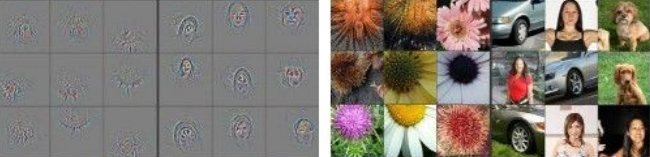
\includegraphics[width = 8in]{../images/Deconv5a}}

\centerline{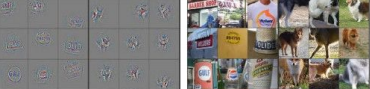
\includegraphics[width = 8in]{../images/Deconv5b}}

\centerline{[Zeigler and Fergus 2013]}

\slide{A Wheel or Face Detector}

The nine strongest stimulators of the ``wheel or face cell'' are the following.

\vfill
\centerline{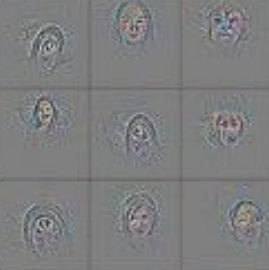
\includegraphics[width = 4.0in]{../images/Deconv6a} \hfill 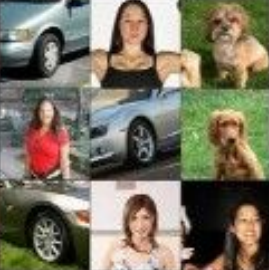
\includegraphics[width=4.0in]{../images/Deconv6b}}

\vfill
\centerline{[Zeigler and Fergus 2013]}

\slide{}
\centerline{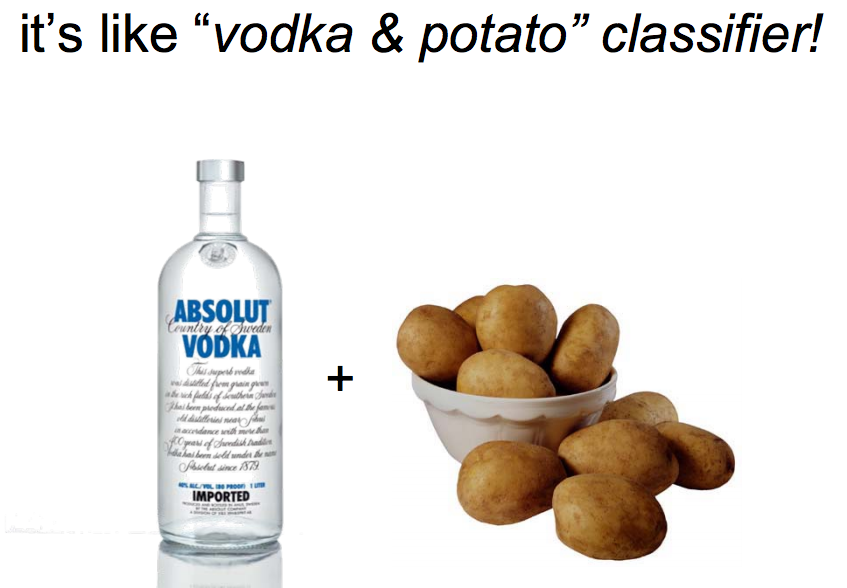
\includegraphics[width = 7.5in]{../images/Potato}}

\centerline{[Alyosho Efros]}

\slideplain{The Kaurnaugh Model of DNNs}

The Karnaugh map, also known as the K-map, is a method to simplify boolean algebra expressions.

\vfil
\centerline{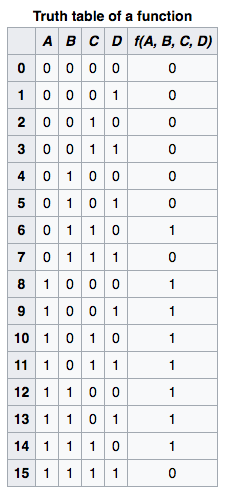
\includegraphics[width = 1.5in]{../images/Kmap1} \hspace{1.0in} 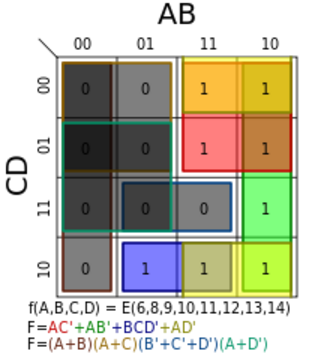
\includegraphics[width=3.0in]{../images/Kmap2}}

\begin{eqnarray*}
  F(A,B,C,D) & = & AC' + AB' + BCD' + AD' \\
  & = & (A+B)(A+C)(B' + C' + D')(A+D')
\end{eqnarray*}

\slideplain{A Kaurnaugh Person Detector}

{\color{red}
  
\centerline{Wheel or Face}

\vfill
\centerline{Hand or Flower \hspace{2.5in} Hand or Flower}

\vfill
\centerline{Leg or Tree  
\includegraphics[height=1.5in]{../images/StickFig} Leg or Tree}
}

\vfill
The set of locally minimal models (circuits) could be vast (exponential) without damaging performance.

\vfill
Is a Boolean circuit a distributed representation?

\slide{The Glass Model of SGD}

Pysical glass (ordinary silica glass) is a metastable state  --- the ground state is quartz crystal.

\vfill
As molten glass cools there is a temperature $T_g$ ($\pm 1$ degrees C) at which it ``solidifies'' (the viscosity becomes huge).

\vfill
This soldification process is very repeatable with a well defined final energy.

\vfill
However, the local optimum achieved is presumably very different for each instance of cooling.

\slide{Identifying Channel Correspondences}

Convergent Learning: Do Different Neural
Networks Learn The Same Representations?, Li eta al., ICLR 2016.

\vfill
Train Alexnet twice with different initializations to get net1 and net2.

\vfill
For each convolution layer, each channel $i$ of net1, and each channel $j$ of net2, compute their correlation.

\vfill
$$\rho_{i,j} = \expect{\frac{(u_i - \mu_i)(u_j- \mu_j)}{\sigma_i \sigma_j}}$$

\slide{Semi-matching and Bipartite matching}

{\bf Semi-matching}: for each $i$ in net1 find the best $j$ in net2:

$$\hat{j}(i) = \argmax_j \rho_{i,j}$$

\vfill
{\bf Biparetitie Matching:} Find the best one-to-one correspondence.

$$\hat{j} = \argmax_{\hat{j}\;\mbox{a bijection}}\;\sum_i \rho_{i,\hat{j}(i)}$$

\vfill
Bipartite matching can be solved by a classical algorithm [Hopcroft and Karp, 1973].  John Hopcroft (age 77) is an author on this ICLR paper.

\slide{Correlations at Layer 1 (Wavelet Layer)}

\centerline{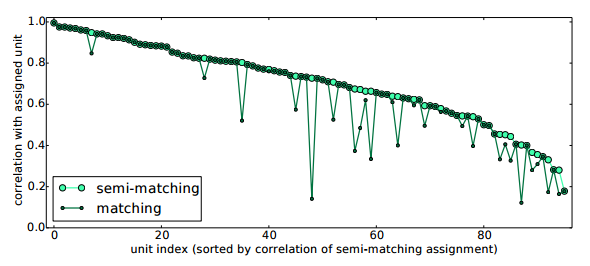
\includegraphics[width = 9in]{../images/Correlations1}}


\slide{Alexnet Layer 1}

\centerline{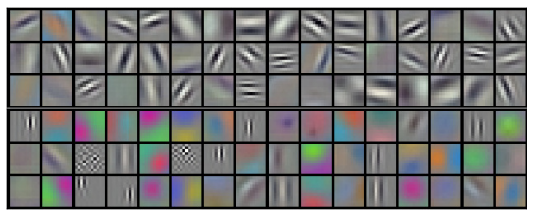
\includegraphics[width = 9.5in]{../images/AlexnetL1}}
\centerline{[Krizhevsky et al.]}

\slide{Best Matches in Layer 1 semi-matching}

\centerline{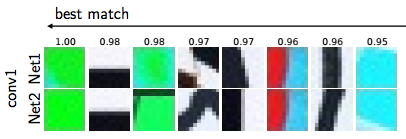
\includegraphics[width = 8in]{../images/Correlations2}}
\centerline{[Li et al.]}

\slide{Worst Matches in Layer 1 semi-matching}

\centerline{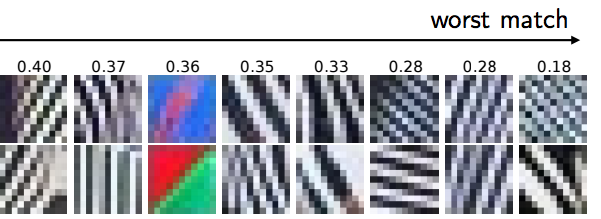
\includegraphics[width = 8in]{../images/Correlations3}}
\centerline{[Li et al.]}

\slide{Layer 1 in Other Networks}

\centerline{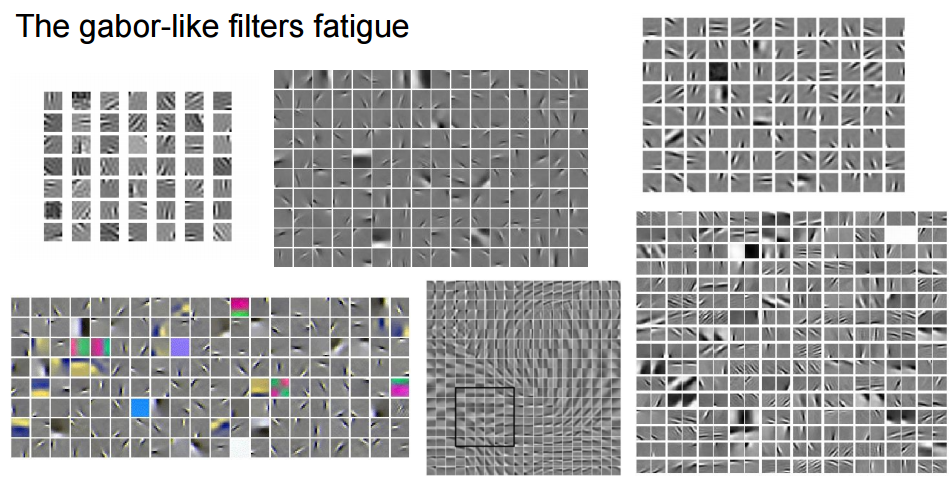
\includegraphics[width = 9.5in]{../images/Filters}}
\centerline{[Stanford CS231]}

\slide{Regression Between Networks at Layer 1}

Model each channel of net1 as a linear combination of channels of net2 using least squares regression.

\vfill
Before the regression each channel is normalized to have zero mean and channel variance.

\vfill
No correlation would yield a {\color{red} square loss of 1.000}.

\vfill
No regularization gives a {\color{red} square loss of 0.170} and uses {\color{red} 96 channels} in each prediction.

\vfill
L1 regularization gives a {\color{red} square loss of 0.235} and uses {\color{red} 4.7 channels} in each prediction.

\slide{Deeper Layers}

\centerline{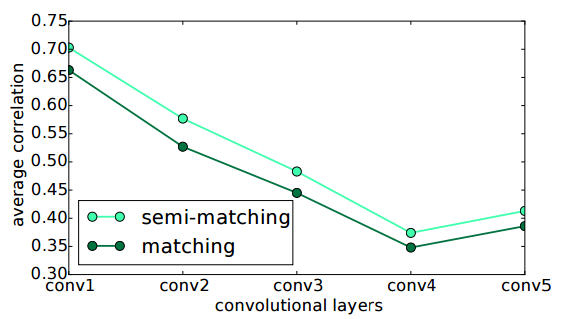
\includegraphics[width = 7.5in]{../images/Correlations4}}

\vfill
In the regression experiment squared error was not significantly reduced at layers 3 through 5 even without regularization. 

\slidetwo{SVCCA Analysis}
{Raghu et al., November 2017}

Consider a matrix $W[i,j]$ used in some model as

\vfill
$$y[i] = \sigma\left(\sum_j W[i,j] x[j] + b[i]]\right)$$

\vfill
We want to understand the meaning of the matrix $W[i,j]$ and the vector $y[I]$.

\slide{SVCCA}

$$y[i] = \sigma\left(\sum_j W[i,j] x[j] + b[i]\right)$$

\vfill
We can collect a set $y[t,I]$  of vectors $y$ computed from $x[t,J]$

\vfill
$$y[t,i] = \sigma\left(\sum_j W[i,j] x[t,j] + b[i]\right)$$

Here $t$ can range over different inputs to the entire network, or different image locations where the filter $W$ is used,
or different times with a single RNN execution.

\slide{PCA on the matrix outputs}

\vfill
We can then perform PCA over the vectors $y[t,I]$ to find a a reduced set of covariance eigenvectors $B[k,I]$.
and represent $y$ by its projection on the eigenvectors.

$$\tilde{y}[t,k] = B[k,I]^\top (y[t,I] - \mu[I])$$

\vfill
PCA can be defined by

\vfill
$$B^* = \argmin_B \sum_t \left|\left|y[t,I] - \mu[I] + \sum_j \;\tilde{y}[t,k]B[k,I]\right|\right|^2$$

\slide{PCA reduction}

Now consider a layer that uses $y[I]$ and the tensor {\bf before the nonlinearity}.

\vfill
$$z[t,v] = \sum_i W'[v,i]y[i] + B'[v]$$

\vfill
This layer can now be redefined to use the $\tilde{y}$

\vfill
$$z[t,v] = \sum_i W''[v,k]\tilde{y}[t,k] + B''[v]$$

\vfill
$$W''[v,k] = \sum_i W'[v,i]B[k,i]$$

\slide{Reduction}

\centerline{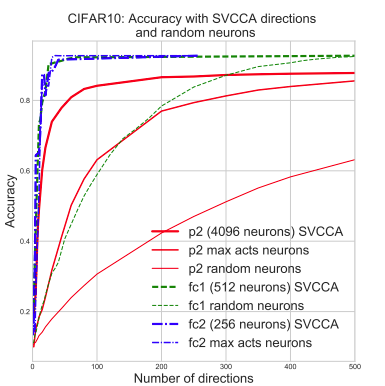
\includegraphics[height=3.5in]{../images/SVCCA}}

\slide{Attention as Explanation}

\centerline{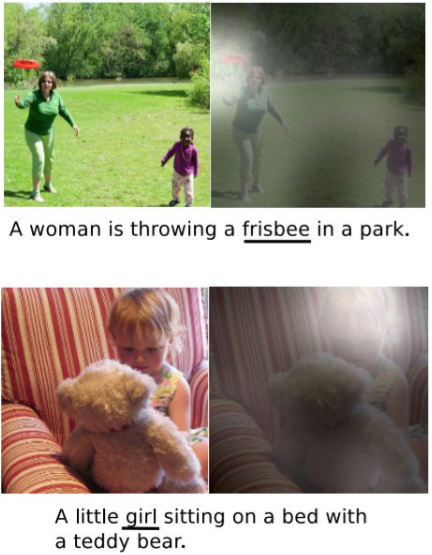
\includegraphics[width = 4in]{../images/AttentionInCaptioning1}}
\centerline{Xu et al. ICML 2015}

\slideplain{Interpretation from Domain Correspondence}

Kushner verliert den Zugang zu streng geheimen Informationen.
$$\Rightarrow$$
Kushner loses access to top-secret intelligence.

\vfill
\centerline{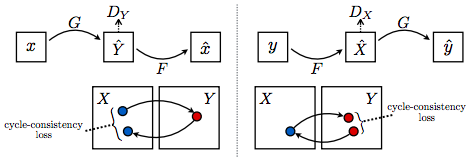
\includegraphics[width = 6.0in]{../images/Cycle2}}

\slide{Causal Models are Explicitly Interpretable}

Flu causes symptoms $x$, $y$ $z$.

\vfill
Strep causes symptoms $x$, $y$, $u$.

\vfill
For the given information on the patient, the prior probability for flu is $\ldots$

\slide{Can Alpha Zero Explain Chess Moves?}

I did $x$ because if I did $y$ they would do $z$ and, in that case, $\ldots$.





\slide{END}





}
\end{document}
